\section{Choosing the right model for the job}
\label{sec:rightmodel}

Heart models of different kinds have been developed for a range of applications and 
\figref{models} shows four heart modeling approaches that emphasize the electric, mechanical, cellular and fluid flow mechanisms of cardiac function. 
Several of these modeling approaches employ over 4 million finite elements or 100,000 ordinary differential equations to describe the dynamics and take several hours to simulate a single cardiac cycle. 
%Several models of the heart have been developed and used in different applications. 
%It should be noted that most models are developed by experiments on animal hearts, in particular pigs.

\emph{Cellular models} describe the generation and spread of electrical action potentials (i.e., voltages) at the molecular-cellular level \cite{PullanBC05_ElectricModelingBook}.
At the cellular level, the flow of charged ions into and out of the cardiac cell is responsible for the change in voltage across the cell membrane. 
%%These \emph{ion channels} have been modeled extensively, typically through ordinary differential equations that relate ion concentrations to electrical currents and voltages.
Cellular models of electrical activity are used to study how activity across ion channels affect the relation between electrical and mechanical behaviors of heart tissue, as well as to study drug therapies that affect the ion channels properties. 
%%While most models were built from first physics principles, some, like the Fenton-Karma model, are a mix of first principles and behavioral approximations which have no physiological basis, but give a good approximation of the shape of the cross-membrane voltage. 
%%Such simplified models have the advantage of being easier to analyze and faster to simulate.

\emph{Anatomical models} are developed using imaging technologies like MRI, and seek to re-create detailed anatomical structures like fiber orientations and the distribution and extent of scar tissue. 
These structures affect the heart's operation by determining muscle contraction and modifying the speed and paths of electrical conduction throughout the heart. 
Thus anatomical models provide a foundation for whole heart modeling efforts that we cover next.
They are also used to simulate the effects of certain medical devices like stents and artificial valves. 

\begin{figure}[t]
		\centering
		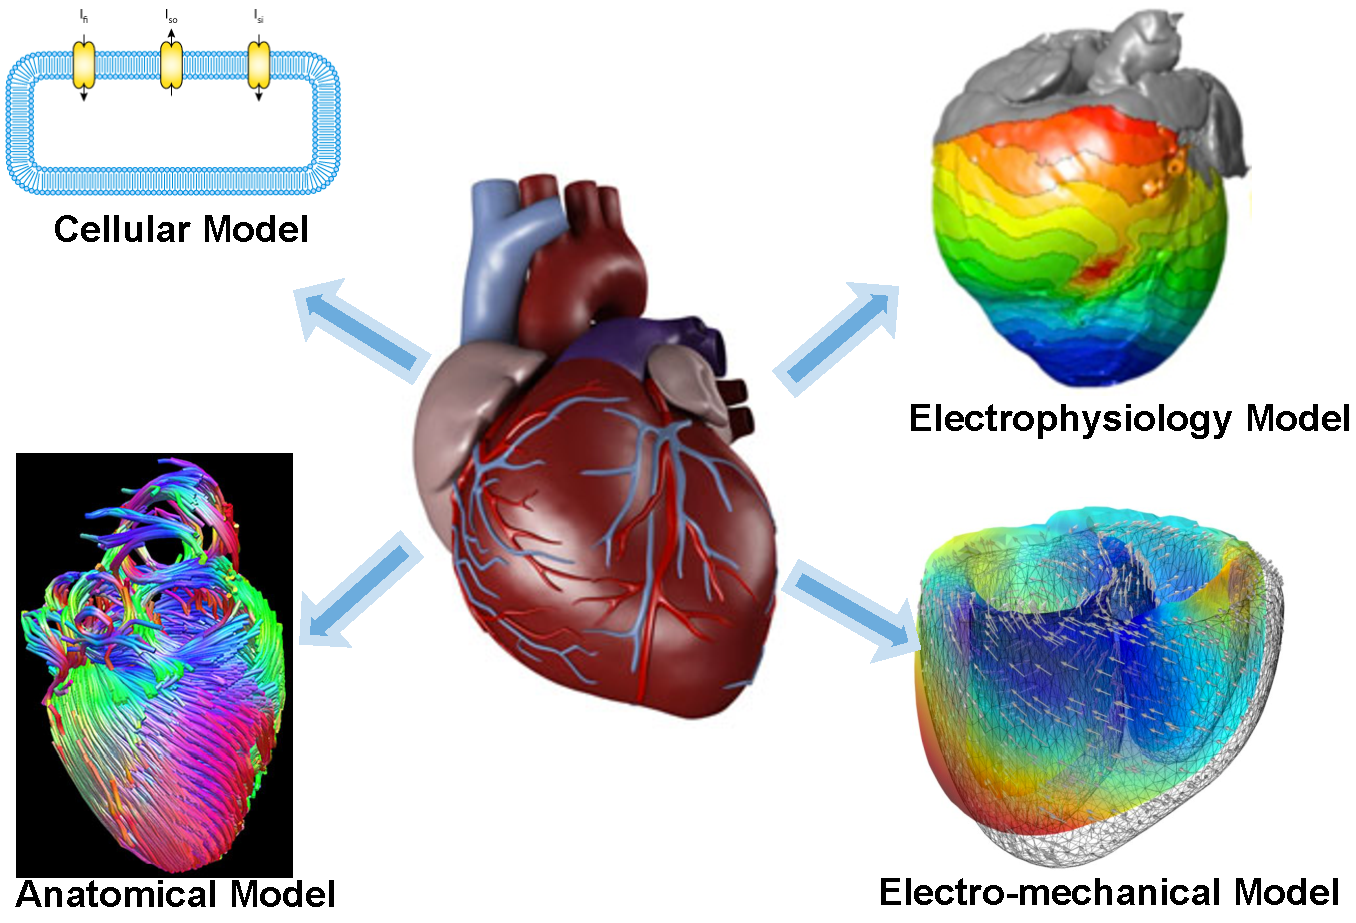
\includegraphics[width=\textwidth]{figs/fig2models.pdf}
		\caption{\small Modelling different phenomena in the heart}
		\label{fig:models}
\end{figure}

\emph{Whole heart models} use a continuum approximation of the cellular models of electrical propagation with the structure obtained from anatomical models. Researchers have developed Partial Differential Equations models of electrical activity in the \emph{whole heart} to analyze the mechanisms of various arrhythmias. 
Researchers at Johns Hopkins \cite{TrayanovaB14_Advances} further used these models to predict the onset of arrhythmias and propose potential therapies. 
Such \emph{electro-mechanical models} help evaluate the mechanical effects of different arrhythmias on blood flow.

\emph{Electrophysiological} (EP) heart models help study the timing properties of the generation and propagation of electrical signals through the electrical conduction system, and can accurately diagnose most arrhythmias. 
%Researchers at Carnegie-Mellon University studied and modeled the heart rate variation
Unlike the aforementioned heart models which are built from the cellular level on up, EP models are developed by conducting a clinical EP testing procedure which is a type or timing analysis of the heart rhythm across the myocardium. EP models are amenable to \emph{model checking}~\cite{model_checking}, a powerful verification technique pioneered in the semiconductor industry.
EP testing is a common method to diagnose arrhythmias: 
a physician inserts catheters with electrodes into the patient's heart through the veins and measures the local electrical activity around the electrodes. 
The physician uses the \emph{patterns} of electrical activity and its timing characteristics to diagnose the heart's condition in terms of arrhythmias, which are derangements to normal timing patterns. 
In particular, electrical timing parameters of action potentials in a tissue region like conduction delay, rest period and refractory period are measured, and any abnormal conduction paths are detected.
%The EP testing studies the timing properties of the generation and propagation of electrical signals through the electrical conduction system, and can accurately diagnose and even treat most arrhythmia. 
\begin{figure}[t]
	\centering
	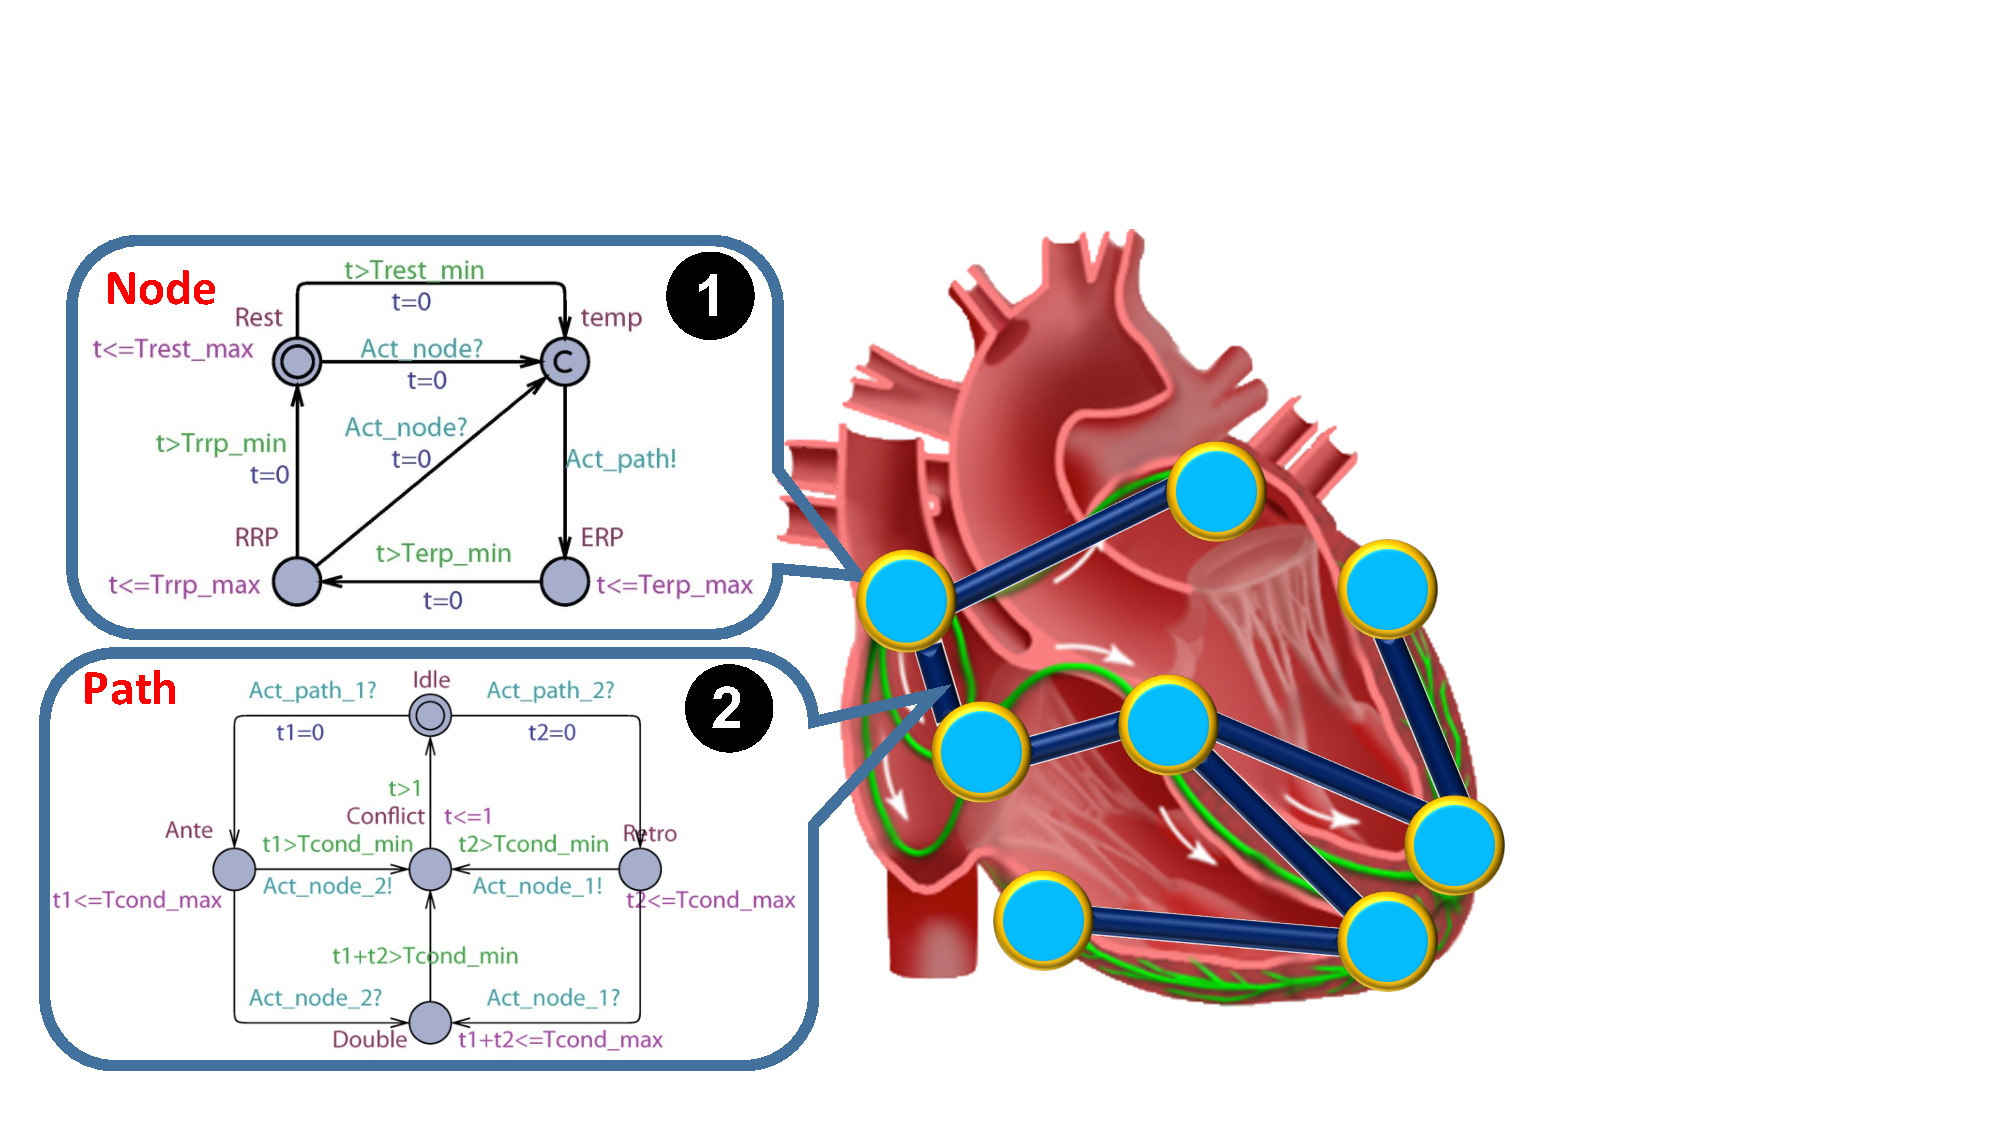
\includegraphics[width=\textwidth]{figs/Pacemaker.pdf}
	\caption{\small Timing of electrical behaviors of the heart are modeled by a network of (1) node and (2) path automata. Each circle is a node automaton which models the generation and blocking of electrical events. Each line is a path automata which models conduction delays between nodes.}
	\label{fig:EP}
\end{figure} 

In \cite{VHM_proc}, researchers from the University of Pennsylvania developed a heart model based on clinical EP testing. 
Since the pacemaker only looks at the \emph{timing} of events as input from only two locations of the heart, this EP model only seeks to model the correct timing of electrical activity in select tissue of the heart.
Specialized tissue like the SA node generates electric events spontaneously and is modeled by Timed Automata known as \emph{node automaton} as shown at Marker 1 in \figref{EP}.
The node automaton models the timing of signal generation, blocking and transmission in heart structures like the AV node. 
The rest of the tissue is abstracted as variable conduction delays as \emph{path automata} between node automata (Marker 2 in \figref{EP}).
Different heart conditions can be modeled by a network of of node/path automata with different  topologies and parameters (\figref{EP}).
Moreover, pacing applied to the heart can be represented as an external activation signal to the node automata.
EP models have been validated by physicians, and have been used for model checking pacemaker software. 

Finally, data-driven models such as~\cite{Bogdan12_fractional} fit (fractional) differential equations directly to measured heart rate without modeling the underlying mechanisms, and are used for optimal control.
